\section{Linux Network Stack}\label{sec:linux_net}
\begin{figure*}
    \centering
    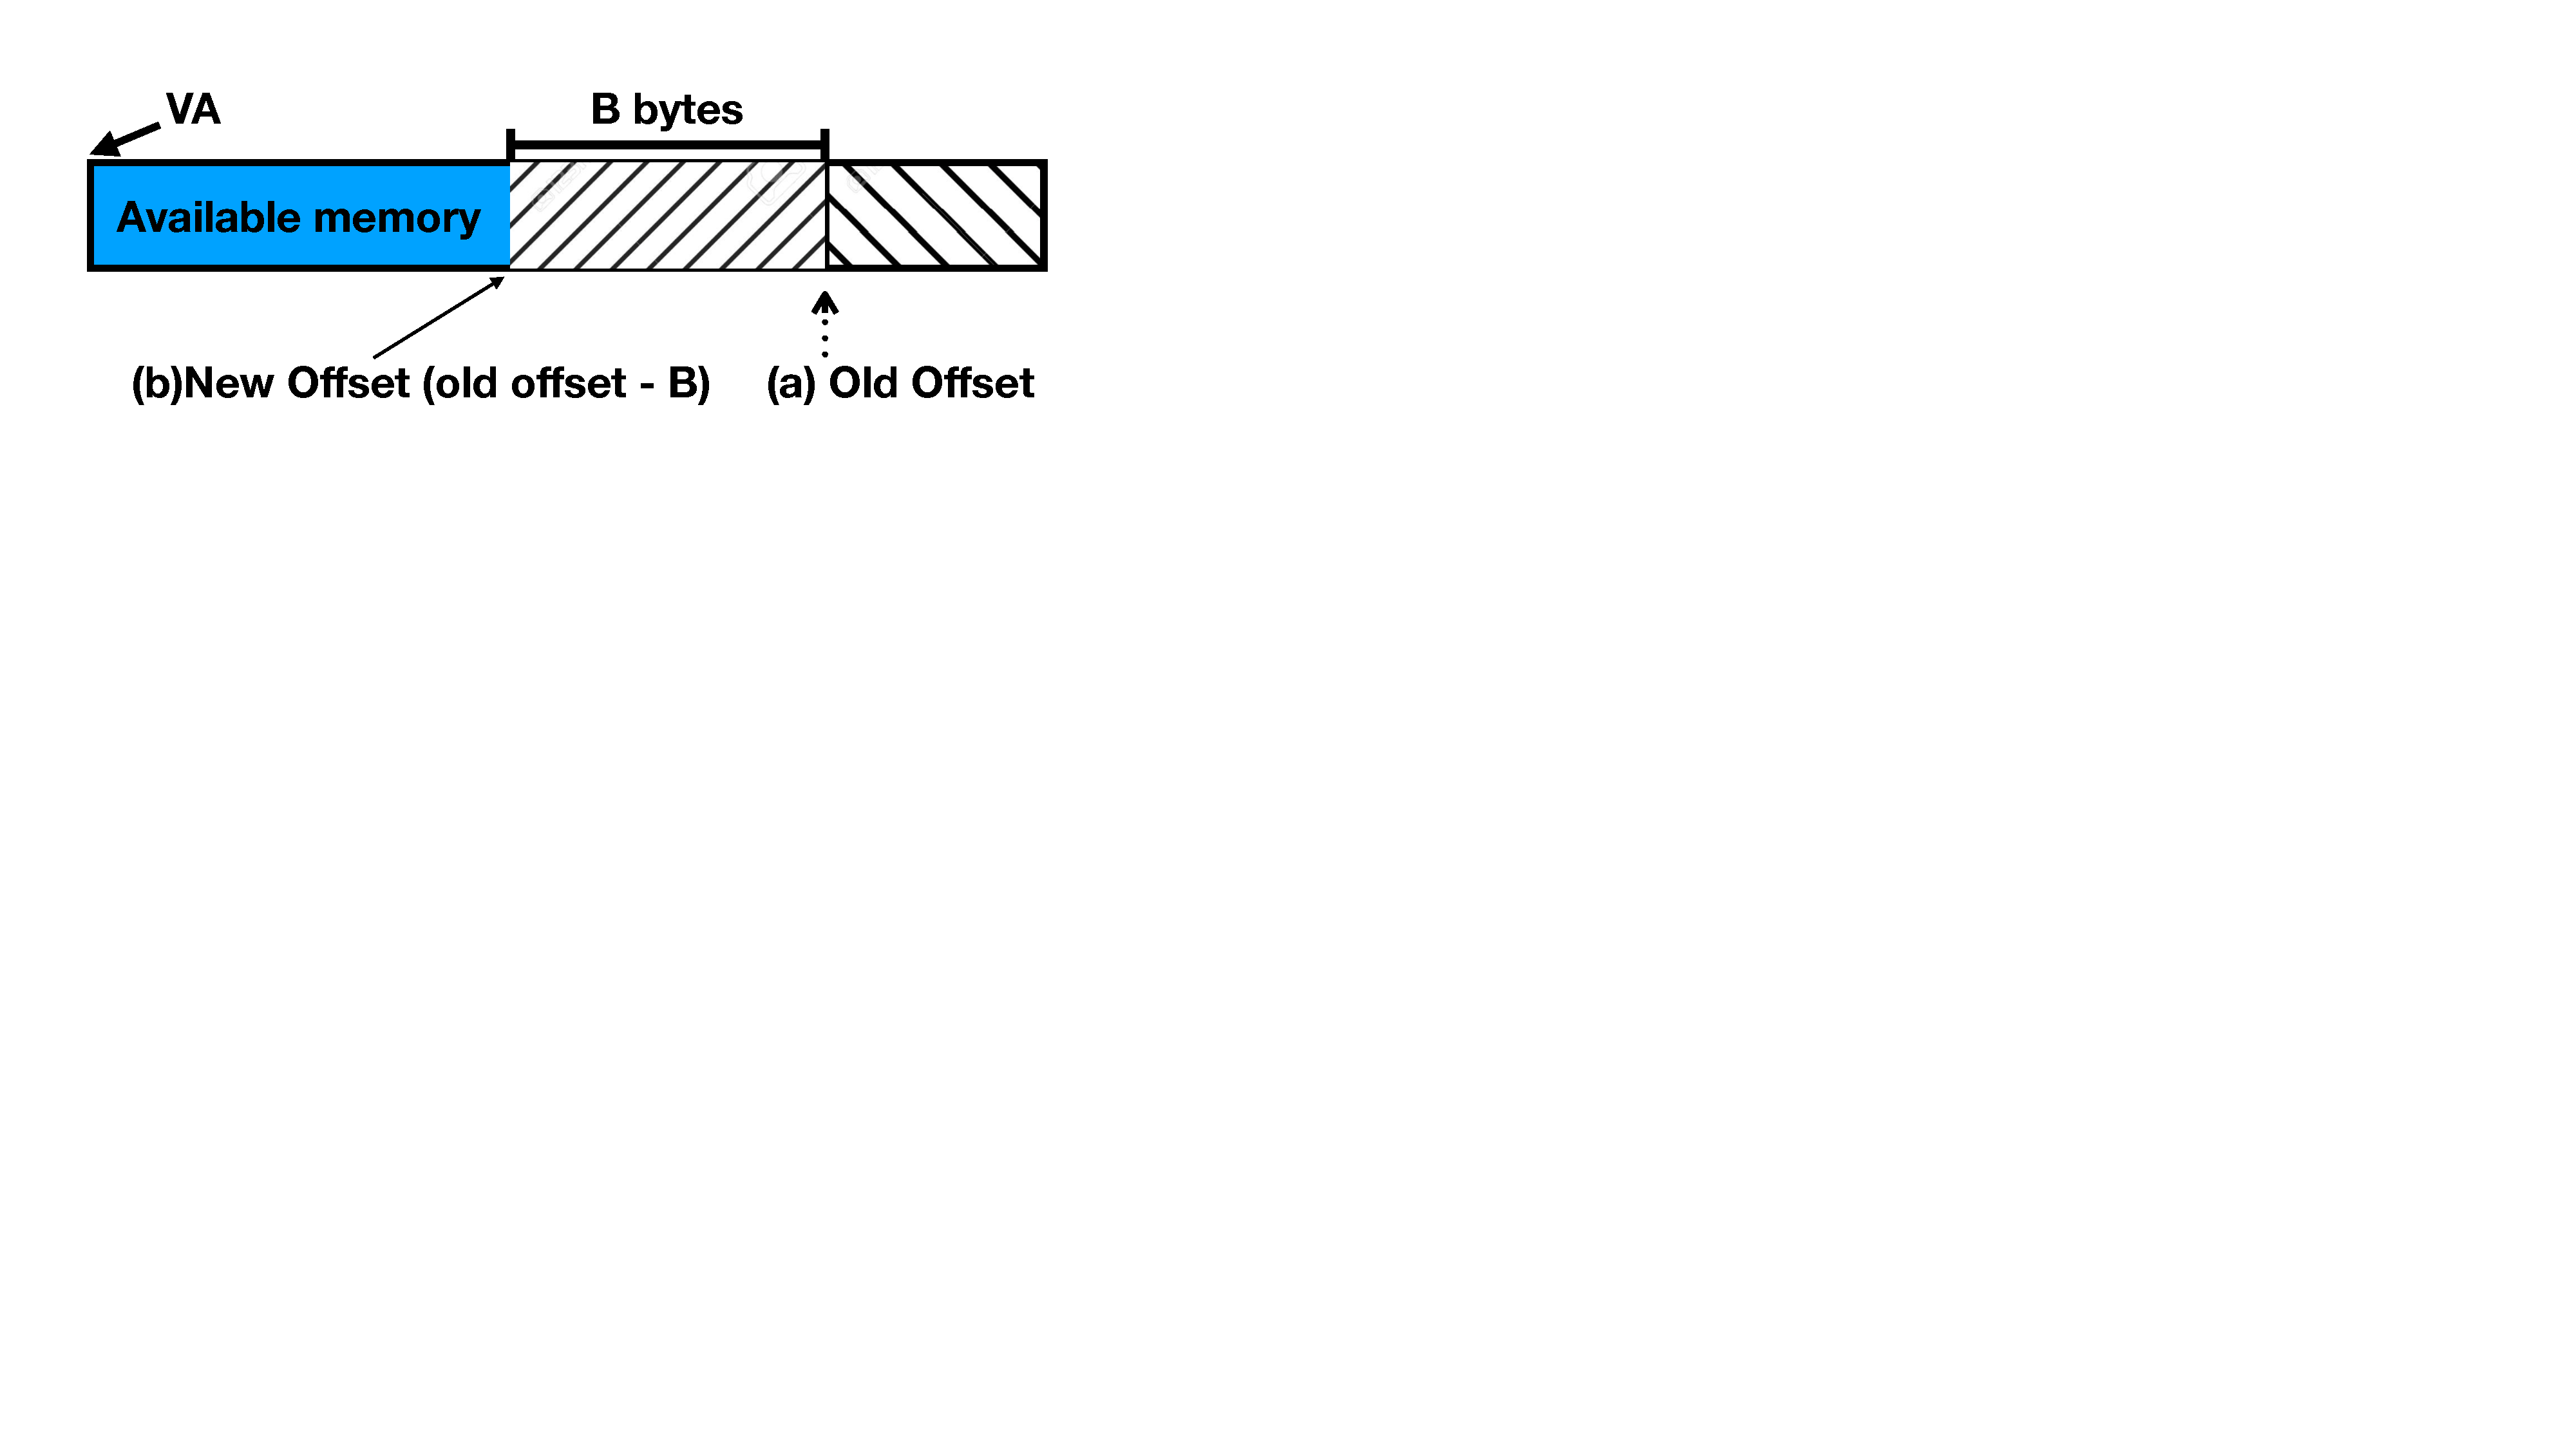
\includegraphics[width=1\linewidth]{figs/page_frag.pdf}
    \caption{Allocation of B bytes from page\_frag}
    \label{fig:page_frags}
\end{figure*}
The previous sections have demonstrated how a malicious device can take over a machine; exploiting the buggy implementation of SBP-2. In this section we explore new attacks on the Linux network stack; where, \textit{Means} and \textit{Opportunity} are harder to come by. 
\subsection{\shinfo}
The sk\_buff is a common data structure that is used in the Linux network stack to hold information  representing a network packet and is used by all network card drivers. Struct \skb holds the metadata of a network packet e.g., its size, associated socket and device and other important information. One of these fields, is a pointer to a data buffer. The data is usually located on a separate page (see Figure \ref{fig:sh_info}). This  separation means that \skb is never (intentionally) mapped to the device; resulting in previous works \cite{thunder} declaring that the Linux network stack is not susceptible to DMA attacks. In reality, the Linux network stack supports packet cloning by copying sk\_buff metadata and letting the new one point to the same data as the old one\cite{drivers2005linux}. To support this data sharing, the \shinfo metadata structure is allocated as part of the data buffer and consequentially is always mapped to the device. Just as in the previous attack, \shinfo is unwittingly mapped for the device with the permissions of the packet i.e., write for RX packets, read for TX packets and in some cases both read and write for XDP/XSK \footnote{\url{https://www.kernel.org/doc/html/v4.18/networking/af_xdp.html}}. This design decision is the \oportunity the malicious device needs. Figure \ref{fig:sh_info} shows how a malicious device can take advantage of a \shinfo to mount an attack on the server with 4 simple steps:
\begin{enumerate}[label=(\alph*)]
    \item an RX \skb and its data buffer are allocated. The data buffer is DMA mapped for the NIC with write access (the write access is to the whole 4K page). 
    \item \textit{destructor\_arg} field in \shinfo is overwritten to point inside the mapped page. Now the \textit{destructor\_arg} is pointing to struct \uarg which is created by the NIC.
    \item \uarg has a callback pointer that is now pointing to the mallicious code that resides on the same page\footnote{In case of NX-bit, its a ROP gadget and a stack}.
    \item when \skb is freed the callback is invoked.
\end{enumerate}
This scenario assumes that the \kva of the mapped page(a.k.a \means) is known to the NIC and that \shinfo will not be overwritten by the CPU. We tackle both issues in this section.

\subsection{Hacking \shinfo}\label{sec:shinfo}
Presumably, a correct use of DMA api by the device driver could easily thwart the attack outlined in Fig \ref{fig:sh_info}. Unmapping the buffer and then initializing \shinfo; should allow the CPU to undo any malicious changes the NIC may have perpetrated. As it turns out, multiple device drivers \footnote{A partial list appears in \ref{apndx:wrong_order}} first create an \skb and only then unmap. Many high speed drivers, avoid unmapping altogether due to the performance penalty of dma\_unamp \cite{MMT16,MSMT18}. These unmapping practices (or bugs) allow the NIC ample opportunity to execute an attack. But even when the order is correct \shinfo is not safe from modifications. The default iommu mode in Linux is deferred protection; and though the unmapp function was called in the right order, the device can still access it via the IOTLB. A security conscious admin may change the default setting to strict. Now the \iova the NIC had for that page is no longer valid. And yet the device can still modify \shinfo. The vulnerability stems from the way \data is allocated. An RX \skb is allocated via the \texttt{napi\_alloc\_skb} or \texttt{netdev\_alloc\_skb} functions\footnote{There are several other options as well, but the principle is the same. \url{https://elixir.bootlin.com/linux/v5.3.8/source/net/core/skbuff.c\#L519}}; these function use a page\_frag to allocate the \data buffer that contains \shinfo. Page\_frag is an efficient method for allocating small buffers of memory. A page\_frag is initialized by allocating a contiguous memory region(usually 32KB), setting a \textit{va} pointer to the start of the region and \texttt{offset} to point to the end. An allocation request for \texttt{B} (See Fig \ref{fig:page_frags}) bytes will subtract \texttt{B} bytes from the \texttt{offset} pointer and return the new value of  \texttt{offset}. 
%\begin{comment}The page\_frag is local to each CPU so there is no contention; page\_frag is replaced with a new one when exhausted.\end{comment} 
This mechanism for memory allocation is very fast, but it also means that consecutive \data buffers will share memory pages. The NIC doesn't need to access the unmapped \iova to modify the \shinfo; it can use the \iova for the next data buffer. The lower 12 bits(the offset on the page) of the \iova  are the same as in the \kva, meaning that the NIC can easily know which \iova overlaps with the previous buffer. In figure \ref{fig:sh_info}, the shaded areas belong to the neighbouring \data buffers. It seems that the only way to secure \shinfo, is to never map it\cite{MSMT18}.
\begin{figure}[h]
    \centering
    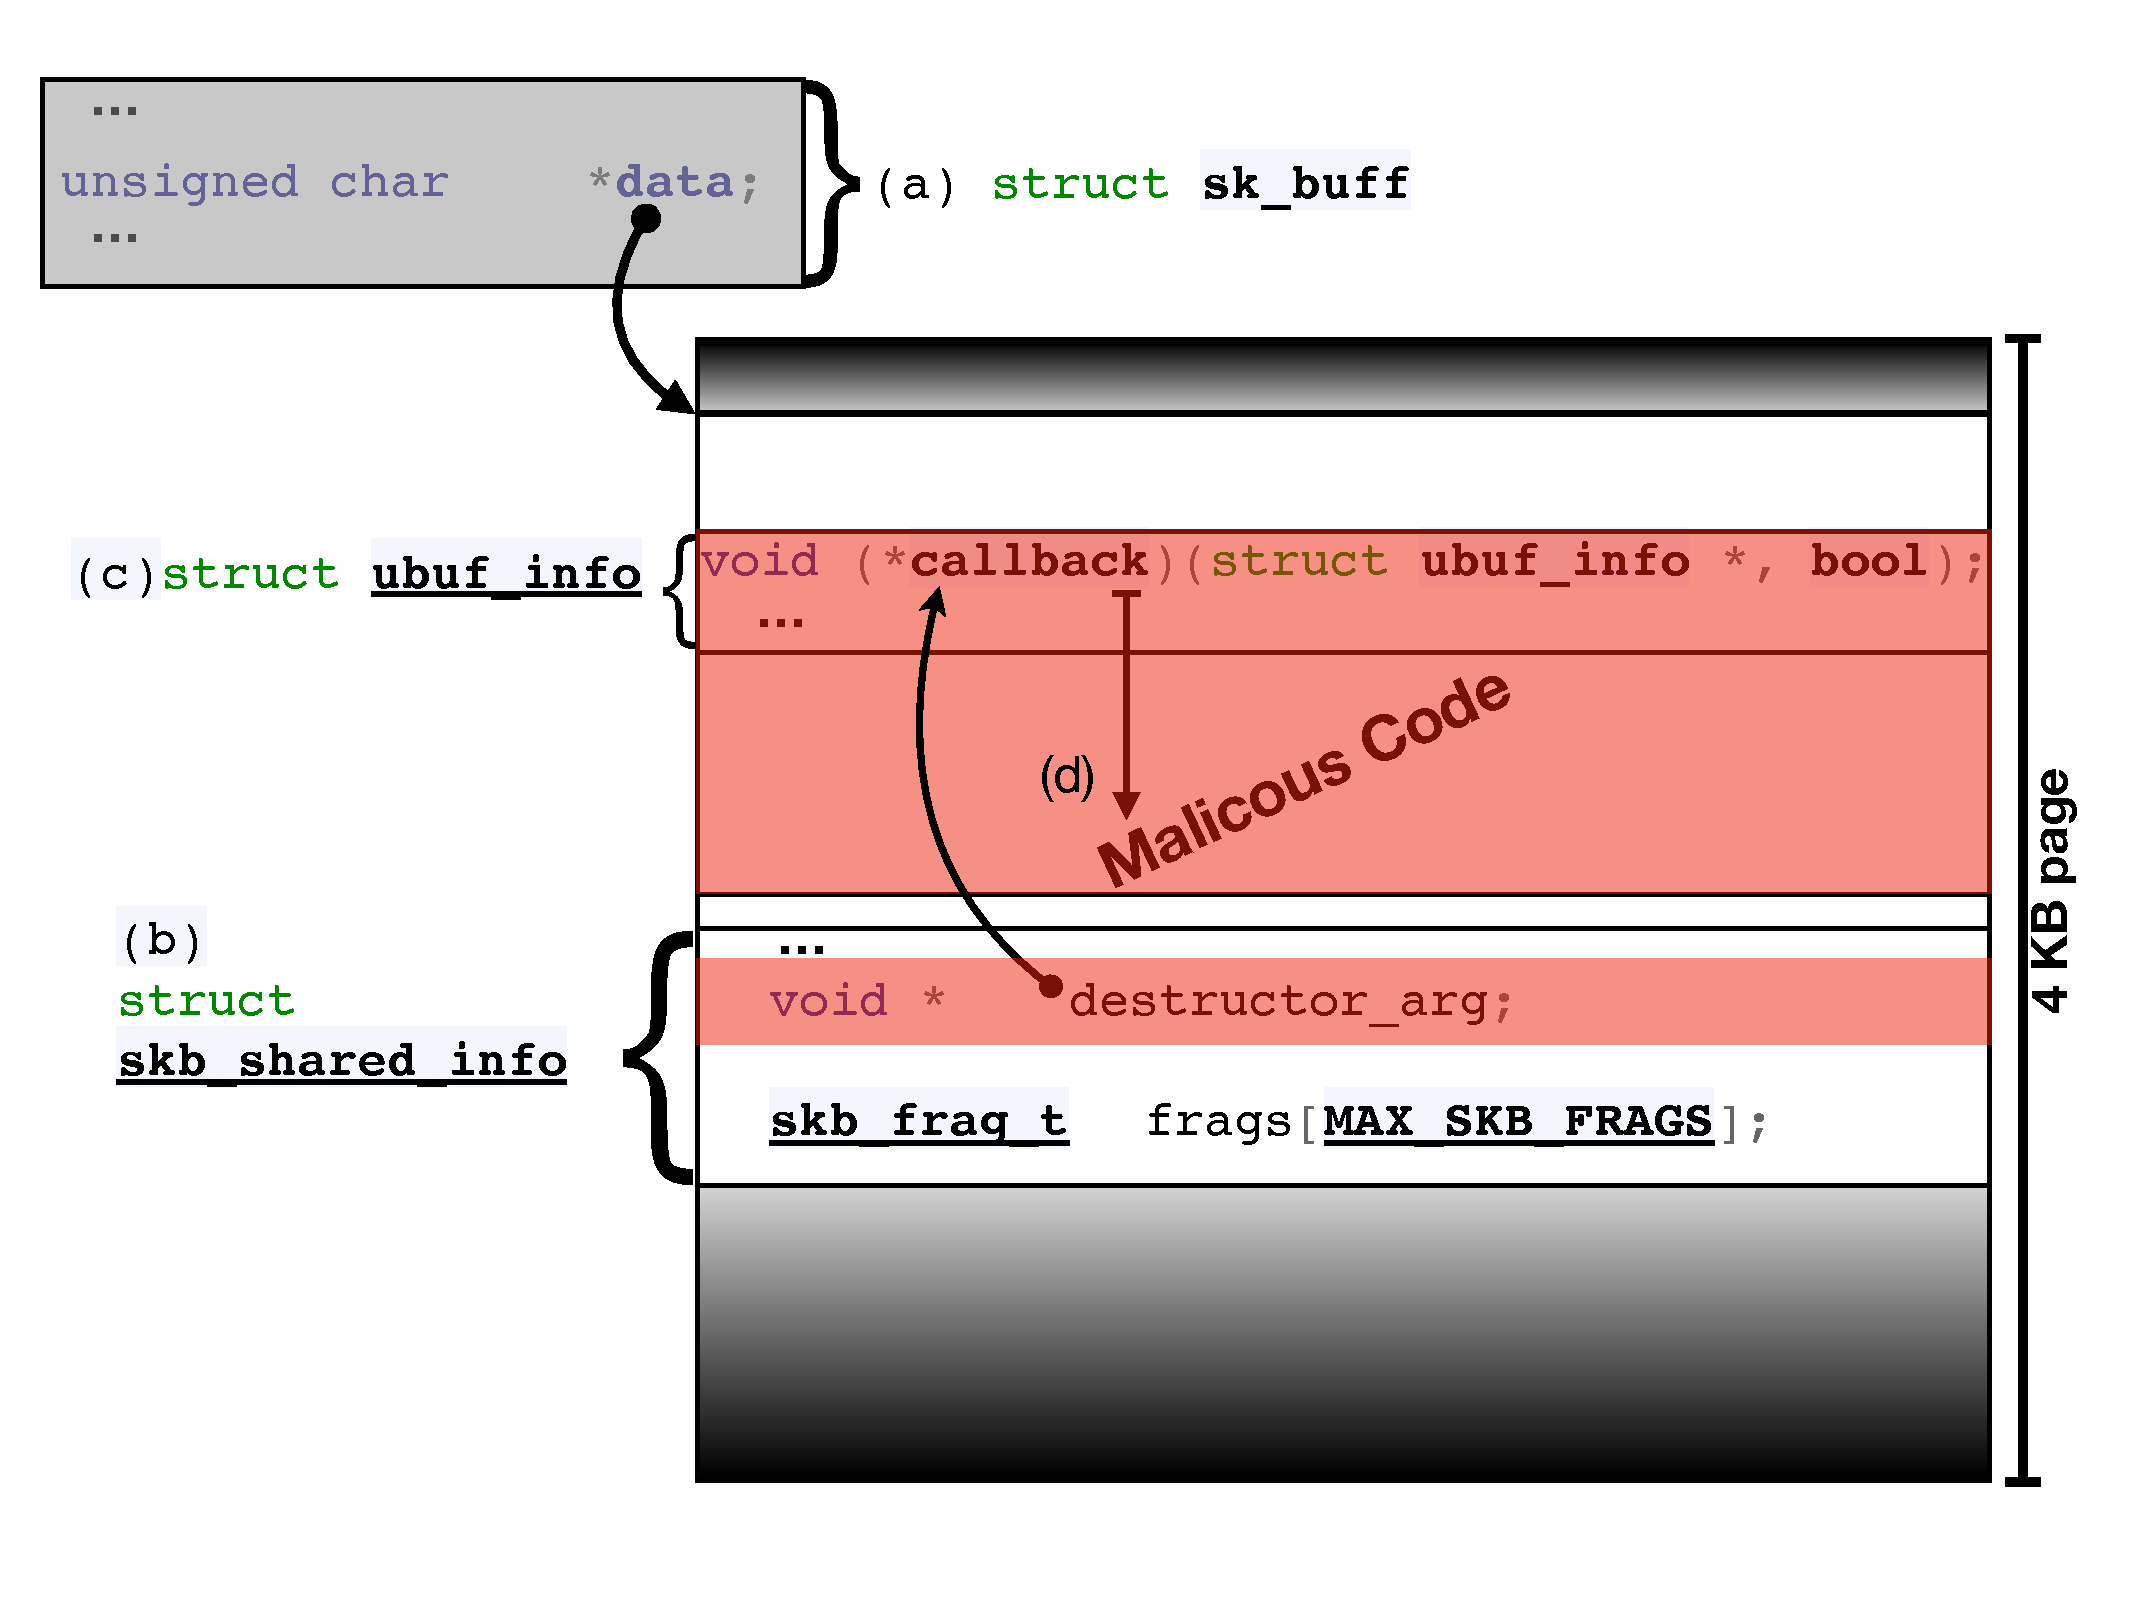
\includegraphics[width=1.2\linewidth]{figs/ubuf.pdf}
    \caption{Using \shinfo to run random code in kernel context.}
    \label{fig:sh_info}
\end{figure}
\subsection{Ring Flod}\label{sec:ringflod}
In \ref{sec:shinfo} we have established that that a malicious NIC has ample opportunity both to create a ROP stack and alter a callback function that will use it. A NIC can calculate a valid kernel\_base pointer(as we have shown in \ref{sec:kaslr}) and other randomized base pointers just by scanning pointers leaked in TX packets\footnote{For example the NIC can spoof a constant stream of pings that will continuously leak kernel pointers}; thus circumventing KASLR. At this point the malicious NIC is still missing the \means to execute an attack.
While the NIC has a \mabaf and a callback function to override; it is missing the \kva to said buffer.
\begin{comment}
%Every RX packet is a possible buffer of malicious code, but the device is only given the buffer iova. The mapping between an iova and its kva is held in the device page table and the device driver meta-data; neither is accessible to the device. On RX the \texttt{struct page} address is filled by the driver(not the KVA) and additionally while we have write access we don't have read access. This means that while the \page address is in a mapped page; we cant read it because its write only. If we could read the \page address; we still wouldn't have the KVA. \newline 
%Luckily for the attacker, the current memory model of x86-64 and ARM Linux servers is SPARSEMEM\_VMEMMAP \cite{mem_model}. Under this memory model the transition between KVA,PFN and \page is trivial once we have the vmem\_base value (Fig \ref{fig:mem_model}). We can guess the value of vmem\_base by looking for kernel pointers in pages mapped for TX packets.\newline
\end{comment}
\newline
The boot process is deterministic; executing the same set of commands, initiating the same modules and allocating the same amount of memory each reboot. While the actual pages each module gets will vary in a multi-core machine due to timing issues, the drift is not expected to be to large. We evaluate this assumptions on a DELL 730 server equiped with a ConnectX-5 NIC, running 256 reboots on Ubuntu 18.04 with kernel 5.0. \textcolor{magenta}{different kernel versions could be better, and three Dell machines}. In the fig\footnote{\textcolor{red}{Please generate table of RingFlod Results}} we show the memory used by each driver and how many of the PFNs repeat in more than 50\% percent of reboots. \textcolor{magenta}{Need to see If we can improve this number}. Thus an adversary that has some knowledge about the physical setup and the kernel version can guess with a high probability a valid \kva for one of the RX pages. Whats left is to fill all the pages with a valid \mabaf and execute an attack as demonstrated in Fig \ref{fig:sh_info}. The callback wont necessarily point back to its own page; but rather to any of the 14K such pages on a 28 core machine\footnote{We assume 1.default RX ring with 1K entries 2.MTU of 1500 where each page is shared by two skbs}. The probability of this attack depends on the driver version and NIC capabilities.For example ,some NICs have a HW LRO capability; where a NIC can aggregate multiple TCP packets into a single TCP packet, larger than MTU (bnx2x and mlx5)\footnote{\textcolor{red}{need reference to capability}}. Drivers configured with these options have a much larger memory footprint and as a result, are much easier to target with a RingFlod attack.
\begin{figure*}
    \centering
    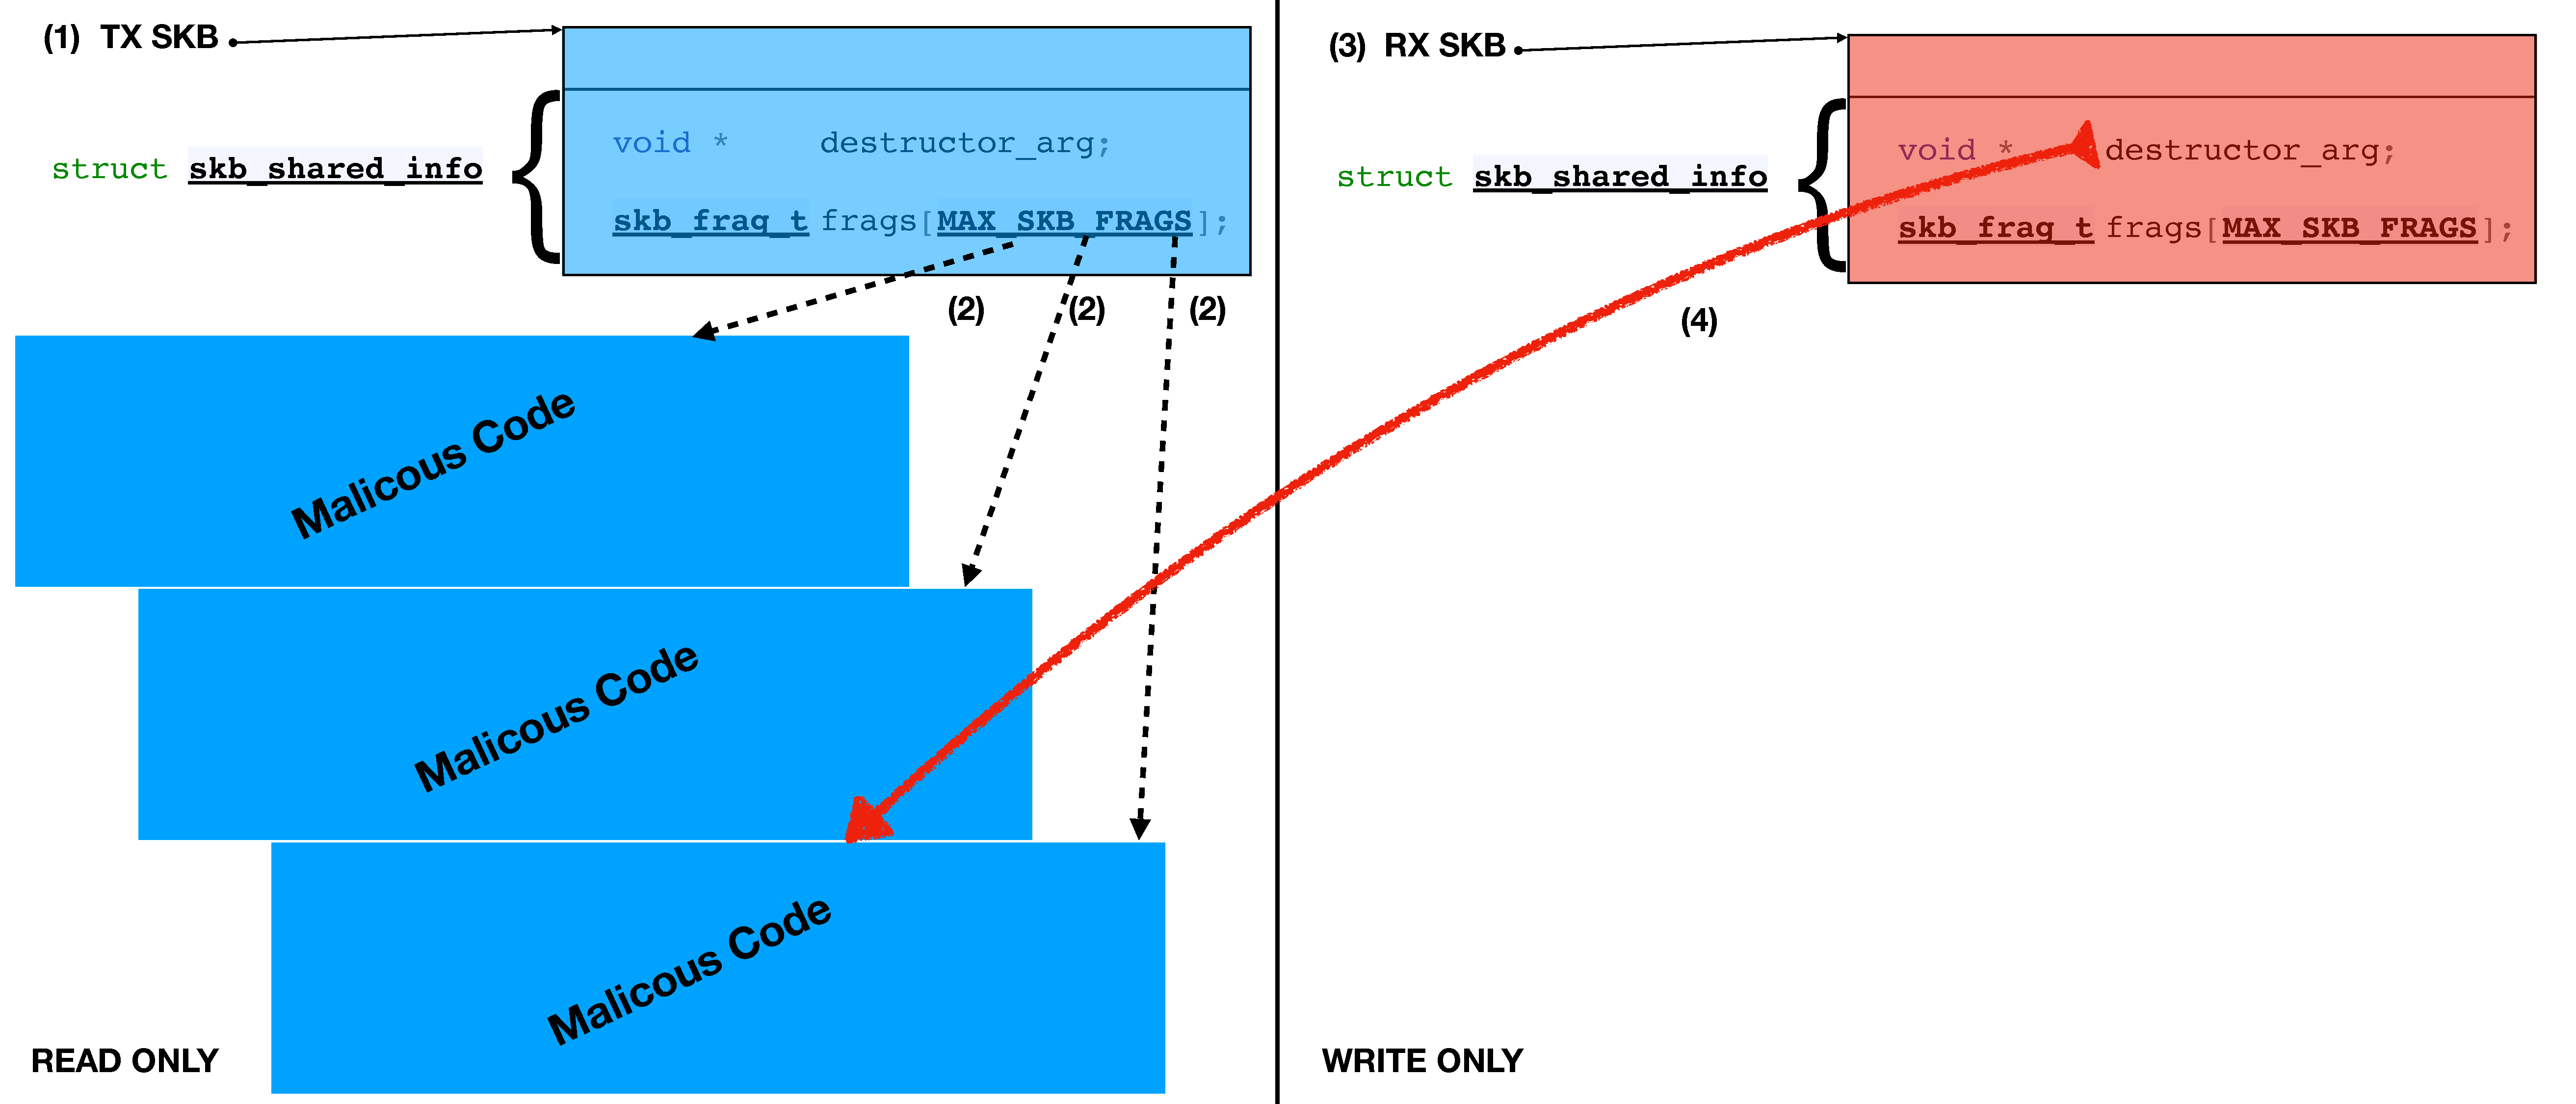
\includegraphics[width=1.1\linewidth]{figs/paylopad_both.pdf}
    \caption{A TX sk\_buff filled with malicious code, used as a \means for a DMA attack}
    \label{fig:payload}
\end{figure*}
\subsection{Poisoned TX}\label{sec:posion}
RingFlod \ref{sec:ringflod} allows a NIC to execute random code with high probability. The prerequisite, is enough information regarding the physical layout of the server and its peripherals\footnote{Other PCIe devices and their location, this all impacts how memory is allocated} and as long as the NIC driver has a high enough memory footprint. When guessing a magic PFN is not an option, we need other \means of computing a valid \kva.\newline
Until now, we have used the sub-page vulnerability of TX packets to break KASLR. As, \shinfo of a TX packet is read only to the NIC, we cant modify its \texttt{destructor\_arg}, but we can learn \page addresses and \texttt{vmemmap\_base}. In addition the fragments them selves are readable to the device. Assuming, an unprivileged accomplice(witing or unwitting) can open a UDP socket in user space; this user could transmit a poisoned buffer. For a ROP attack (where we need the Kernel text offsets) we assume the NIC has spoofed an UDP packet with poisoned content for the accomplice to send. Once an accomplice sends the packet the NIC can execute the attack in 4 simple steps (Fig \ref{fig:payload}):
\begin{enumerate}
    \item The TX \data and the fragments are mapped for the NIC to read.
    \item The NIC identifies the poisoned buffer and translates \page to \kva.
    \item The NIC spoofs an RX packet, and delays the completion notification of the TX packets (we don't want the \mabaf to be released prematurely).
    \item The NIC overwrites \shinfo with the \kva retrieved in step 2. 
\end{enumerate}
%But if the fragments hold malicious content; its all the malicious NIC needs for a successful attack. The readable \shinfo holds a \kva for a \page. This both allows the NIC to break KASLR and gives a \kva\footnote{\textcolor{magenta}{Do show exactly what are the KASLR bits and how you break it}} of a valid \mabaf. To implement the attack the NIC will generate an RX packet and fill the \uarg address from the calculated \kva.
%The NIC will hold off on the TX completion event in order to make sure that \kva is not freed by the TX completion handler; before the poisoned RX packet is processed. A TX completion event that fails to appear in due time, will trigger a TX T/O error that will flush all buffers; the T/O is set by the driver usually to 5 seconds, which is enough to implement an attack.\newline
In this scenario the attacker doesn't need any prior knowledge of the kernel or the hardware. The only assumption is that there is an accomplice (witting or unwitting) that can open a socket in user-space. For that matter, a socket in user-space of a guest machine; making any cloud VM or a Proxy server a valid intrusion tool in the presence of a malicious device.\newline
Having an accomplice, in the form of an unprivileged user provides other vectors of attack as well. In addition to running ROP attacks; the NIC can also leak the content of arbitrary memory pages to the user. Assuming that the NIC has write access to \shinfo after it has been sent up the network stack. For example, in case of deferred protection or when pool\_page is used (see \ref{sec:xdp}). The NIC can modify the \page address in the \texttt{frag} entries, and so let the Linux network stack copy the context of arbitrary memory pages to an unprivileged user.

\subsection{Forward Thinking}
In some situations, an accomplice will not be available. Packet forwarding functionality is usually disabled by default in Linux machines. But some Linux servers may function as a router or an L3 load balancer; these machines will have packet forwarding enabled. In this scenario instead of waiting for an accomplice to send a poisoned packet; the NIC can independently generate an RX packet to a destination that is reachable from the server. For a TCP connection, the Linux kernel will attempt to aggregate multiple TCP segments into a single large packet\footnote{Generic Receive offload,\url{https://access.redhat.com/documentation/en-us/red_hat_enterprise_linux/6/html/performance_tuning_guide/network-nic-offloads}}. This packet will then be forwarded and become a TX packet. A TX packet that can be used as described in the previous attack (\ref{sec:posion}) Fig \ref{fig:payload}. \newline
Packet forwarding, also opens up additional attack options. Instead of sending a TCP packet and letting the GRO layer fill in the \texttt{frags} information. The NIC can generate a small UDP packet and fill in the \texttt{frags} array with any arbitrary \page on the system. This will make the driver map these pages with DMA\_TO\_DEVICE; providing read access to any page on the system to the NIC. The mlx5\_core, the driver of our NIC will map all the frags in \shinfo, w/o checking the actual packet length.  

\begin{figure*}
    \centering
    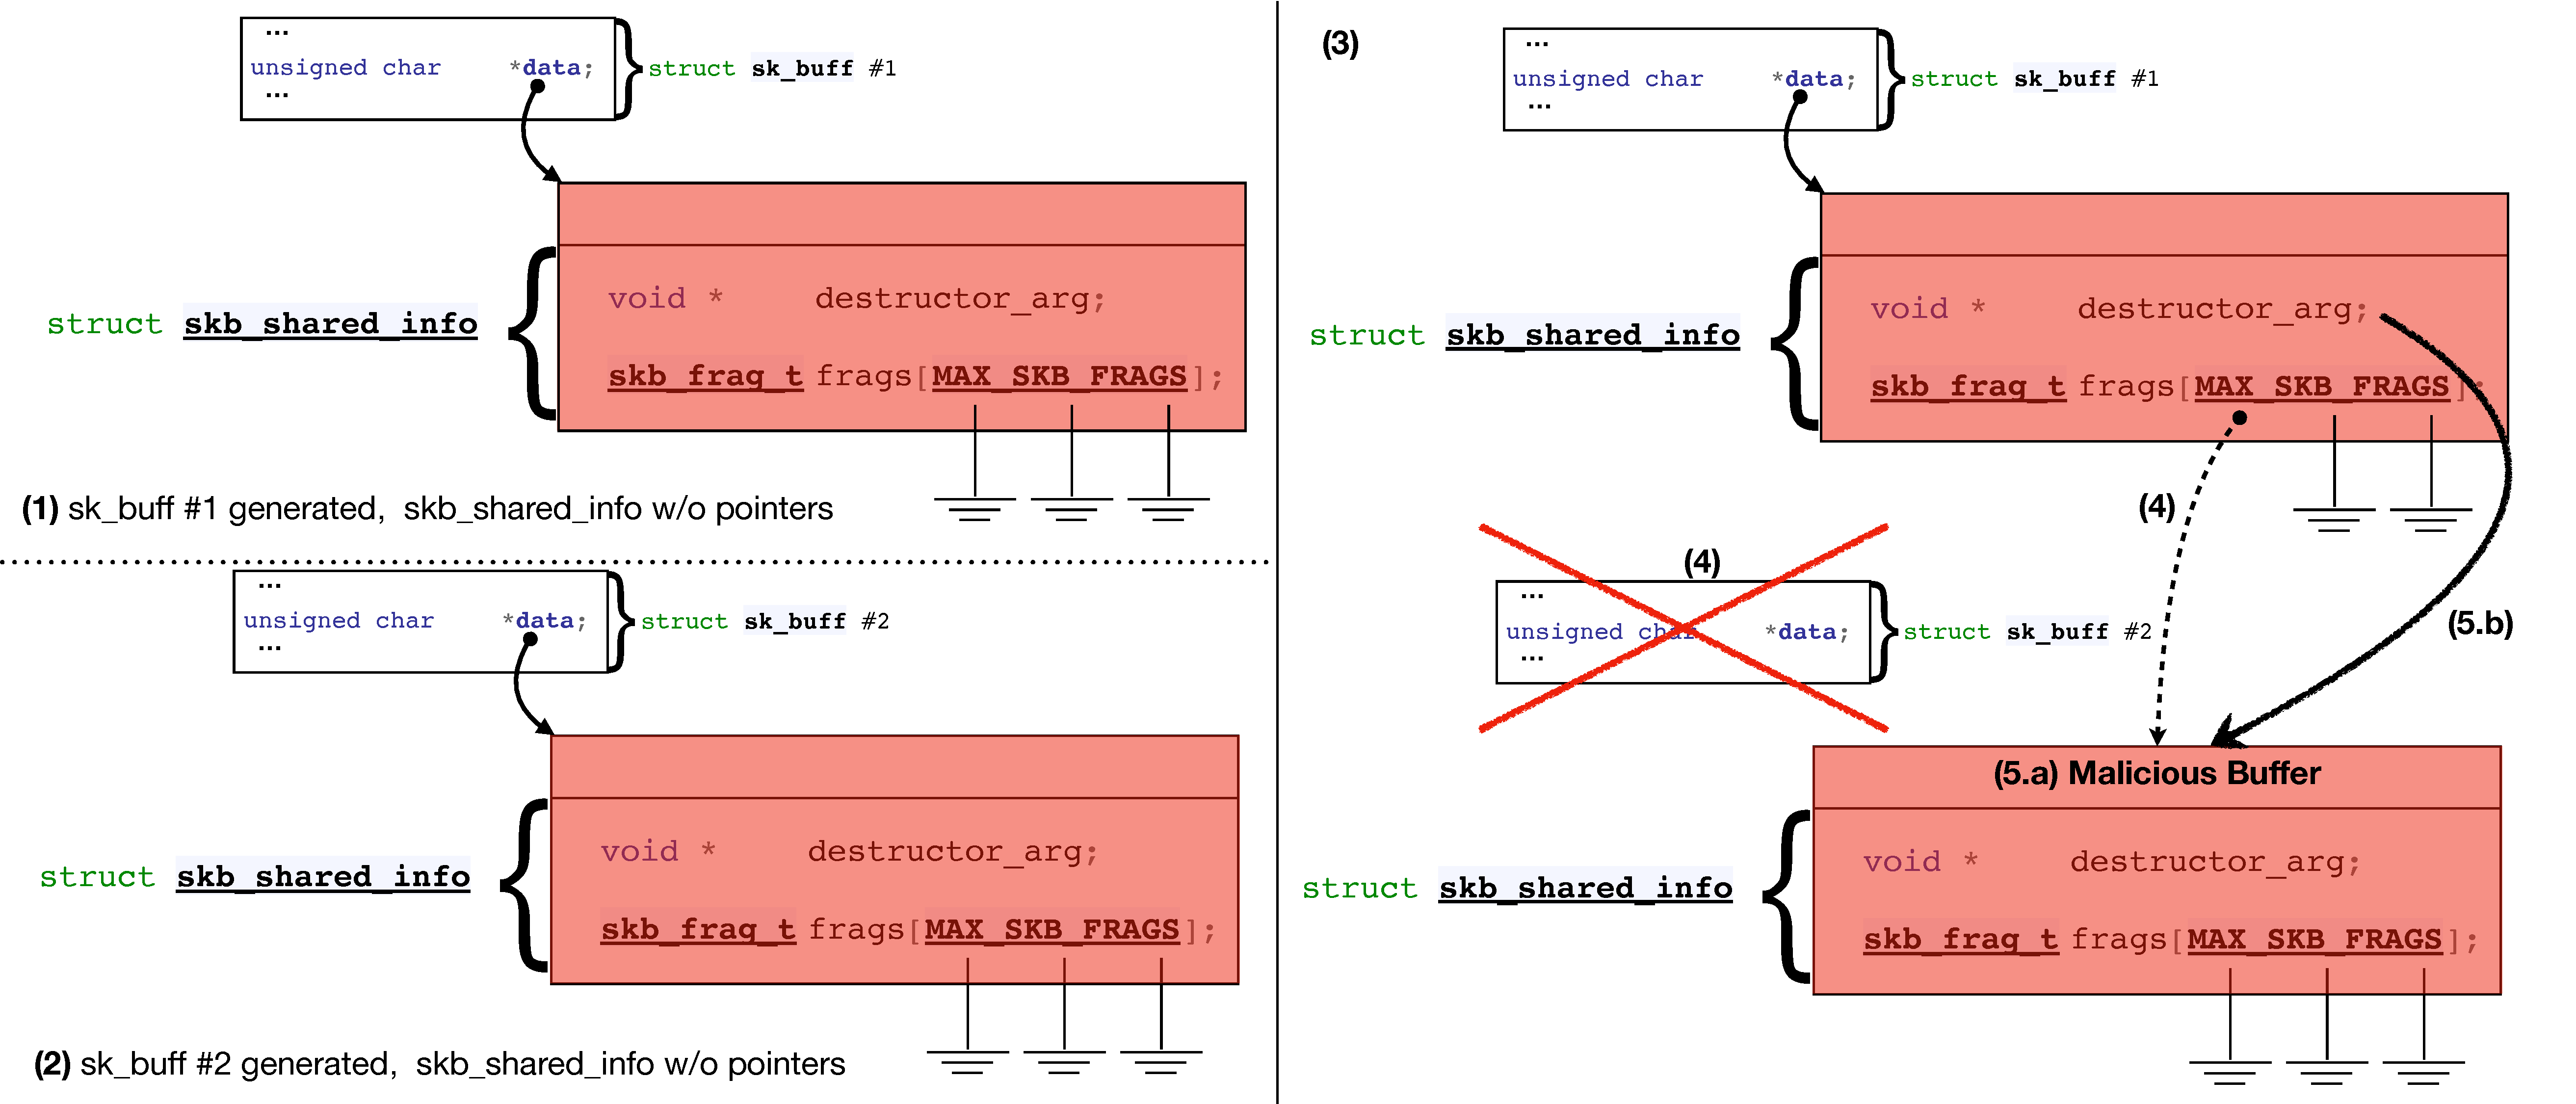
\includegraphics[width=1.1\linewidth]{figs/gro_generation.pdf}
    \caption{An RX sk\_buff after GRO, used as a \means for a DMA attack}
    \label{fig:gro}
\end{figure*}

\subsection{XDP}\label{sec:xdp}
XDP\footnote{\url{https://www.iovisor.org/technology/xdp}} provides a way for users to add custom handling to RX buffers with little overhead. Use cases, include DDOs mitigation for security and Forwarding and load balancing; for the latter the RX buffers need to be also readable to the NIC. As a result all RX buffers are mapped with DMA\_BIDIRECTIONAL rather than the usual DMA\_FROM device. Additionally, in an attempt to avoid performance penalties from memory allocation \cite{xdp} and DMA mapping/unmapping; the RX buffers are reused in a page\_pool\cite{page_pool}. These, pages are never unmapped, and remain accessible to the device both for read and write through out the pools existence (read forever). In this section we will focus on the latest mlx5\_core drivers of the NICs we have on our setup. Other drivers with XDP patches show similar behaviour\footnote{\textcolor{red}{Add a list of drivers to Appendix}}. It is important to note, that a DMA-page pool mechanism is not an inherently bad idea when implemented with caution\cite{MSMT18}. Also, its important to note that the mlx5\_core driver has two modes of operation; linear - where an skb is built around an RX buffer and non-linear where the driver is is filling up the \texttt{frags} of \shinfo. The former is the default, and the later is actually secure. The non-linear mode of opeation is secure because \shinfo is never accessible to the device; and thus the NIC never has the \oportunity to attack.\newline
In linear mode the NIC has both read, and write access to \shinfo; this additional read capability allows the NIC to run and exploit in 4 steps (Fig \ref{fig:gro}):
\begin{enumerate}
    \item An RX \skb is generated, its part of a TCP stream. \shinfo is initialised by the CPU and the \texttt{frags} are filled with NULL pointers.
    \item A second RX \skb is generated and its part of the same TCP stream.
    \item The second \skb is coalesced with the first packet. The \skb is freed and the \data is added as a \texttt{frag} to the first \skb.
    \item The NIC reads the updated \texttt{frag} field, translates the \page address to a valid \kva and finally fills the \texttt{destructor\_arg} field. Creating a poisoned \skb like in Fig \ref{fig:sh_info}.
\end{enumerate}
The difference between this flow and a regular receive flow is the additional read capability the NIC has due to XDP.
\begin{comment}
%The linear skbs in mlx5 are mapping sh\_info as BI\_DIR, need to see when linear used vs non-linear and to check othe XDP drivers. When sh\_info is mapped BI\_DIR its all we need to attack.\newline It seems linear skb (No (HW?)LRO and MTU<1500 : verify with experimnt or Boris) means no frags, while \begin{enumerate}
%    \item build\_skb is used on a mapped page
%    \item page is unmapped in a deferred way, regardless of iommu policy; a driver hack.
%\end{enumerate} 
 \begin{enumerate}
    \item skb\_try\_coalesce
    \item SW LRO/GRO
\end{enumerate}.
\newline
\textcolor{magenta}{In addition reviewing other drivers for the intersection of DMA\_BIDIR \^ (skb\_add\_rx\_frag||skb\_fill\_page\_descriptor)}
\end{comment}
